\documentclass[12pt]{beamer}
\usepackage[utf8x]{inputenc}
\usepackage{ucs}
\usepackage{amsmath}
\usepackage{amsfonts}
\usepackage{amssymb}
\usepackage{graphicx}
\usepackage{colortbl}
\usepackage{fontawesome}

\mode<presentation>{}
\setbeamertemplate{footline}[frame number]{}
\setbeamertemplate{navigation symbols}{}

\AtBeginSection[]
  {
    \ifnum \value{framenumber}>0
      \begin{frame}<beamer>
      \frametitle{Outline}
      \tableofcontents[currentsection]
      \end{frame}
    \else
    \fi
  }


\author{Mikhail Shugay, PhD}
\title{T-cell repertoire annotation and motif discovery}
\subtitle{A RepSeq data analysis tutorial in R}
\institute[Skoltech]{\texttt {Skolkovo Institute of Science and Technology}}
\date{29 October 2018, 2\textsuperscript{nd} SCAIR meeting}

\begin{document}

\maketitle

\section{Introduction}

\begin{frame}{Aims of this tutorial}
\textbf{Aim1} Learn how to infer T-cells specific to certain epitopes and extract T-cell receptor (TCR) sequence motifs from high-throughput sequencing data (RepSeq).\\~\

\textbf{Aim2} Get familiar with \texttt{VDJdb} database, \texttt{VDJtools} software and some useful R templates for TCR sequence analysis.\\~\

\textbf{Disclaimer} This tutorial will not cover RepSeq data processing and basic\footnote{Repertoire diversity analysis, segment usage, etc. See \href{https://vdjtools-doc.readthedocs.io/en/master/examples.html}{\textbf{Examples} section of \texttt{VDJtools} docs} for this.} analysis.
\end{frame}

\begin{frame}{VDJdb database}
\begin{columns}
\column{0.45\textwidth}
VDJdb is a curated database of T-cell receptor sequences of known antigen specificity that can be accessed at \url{http://vdjdb.cdr3.net}
\column{0.55\textwidth}
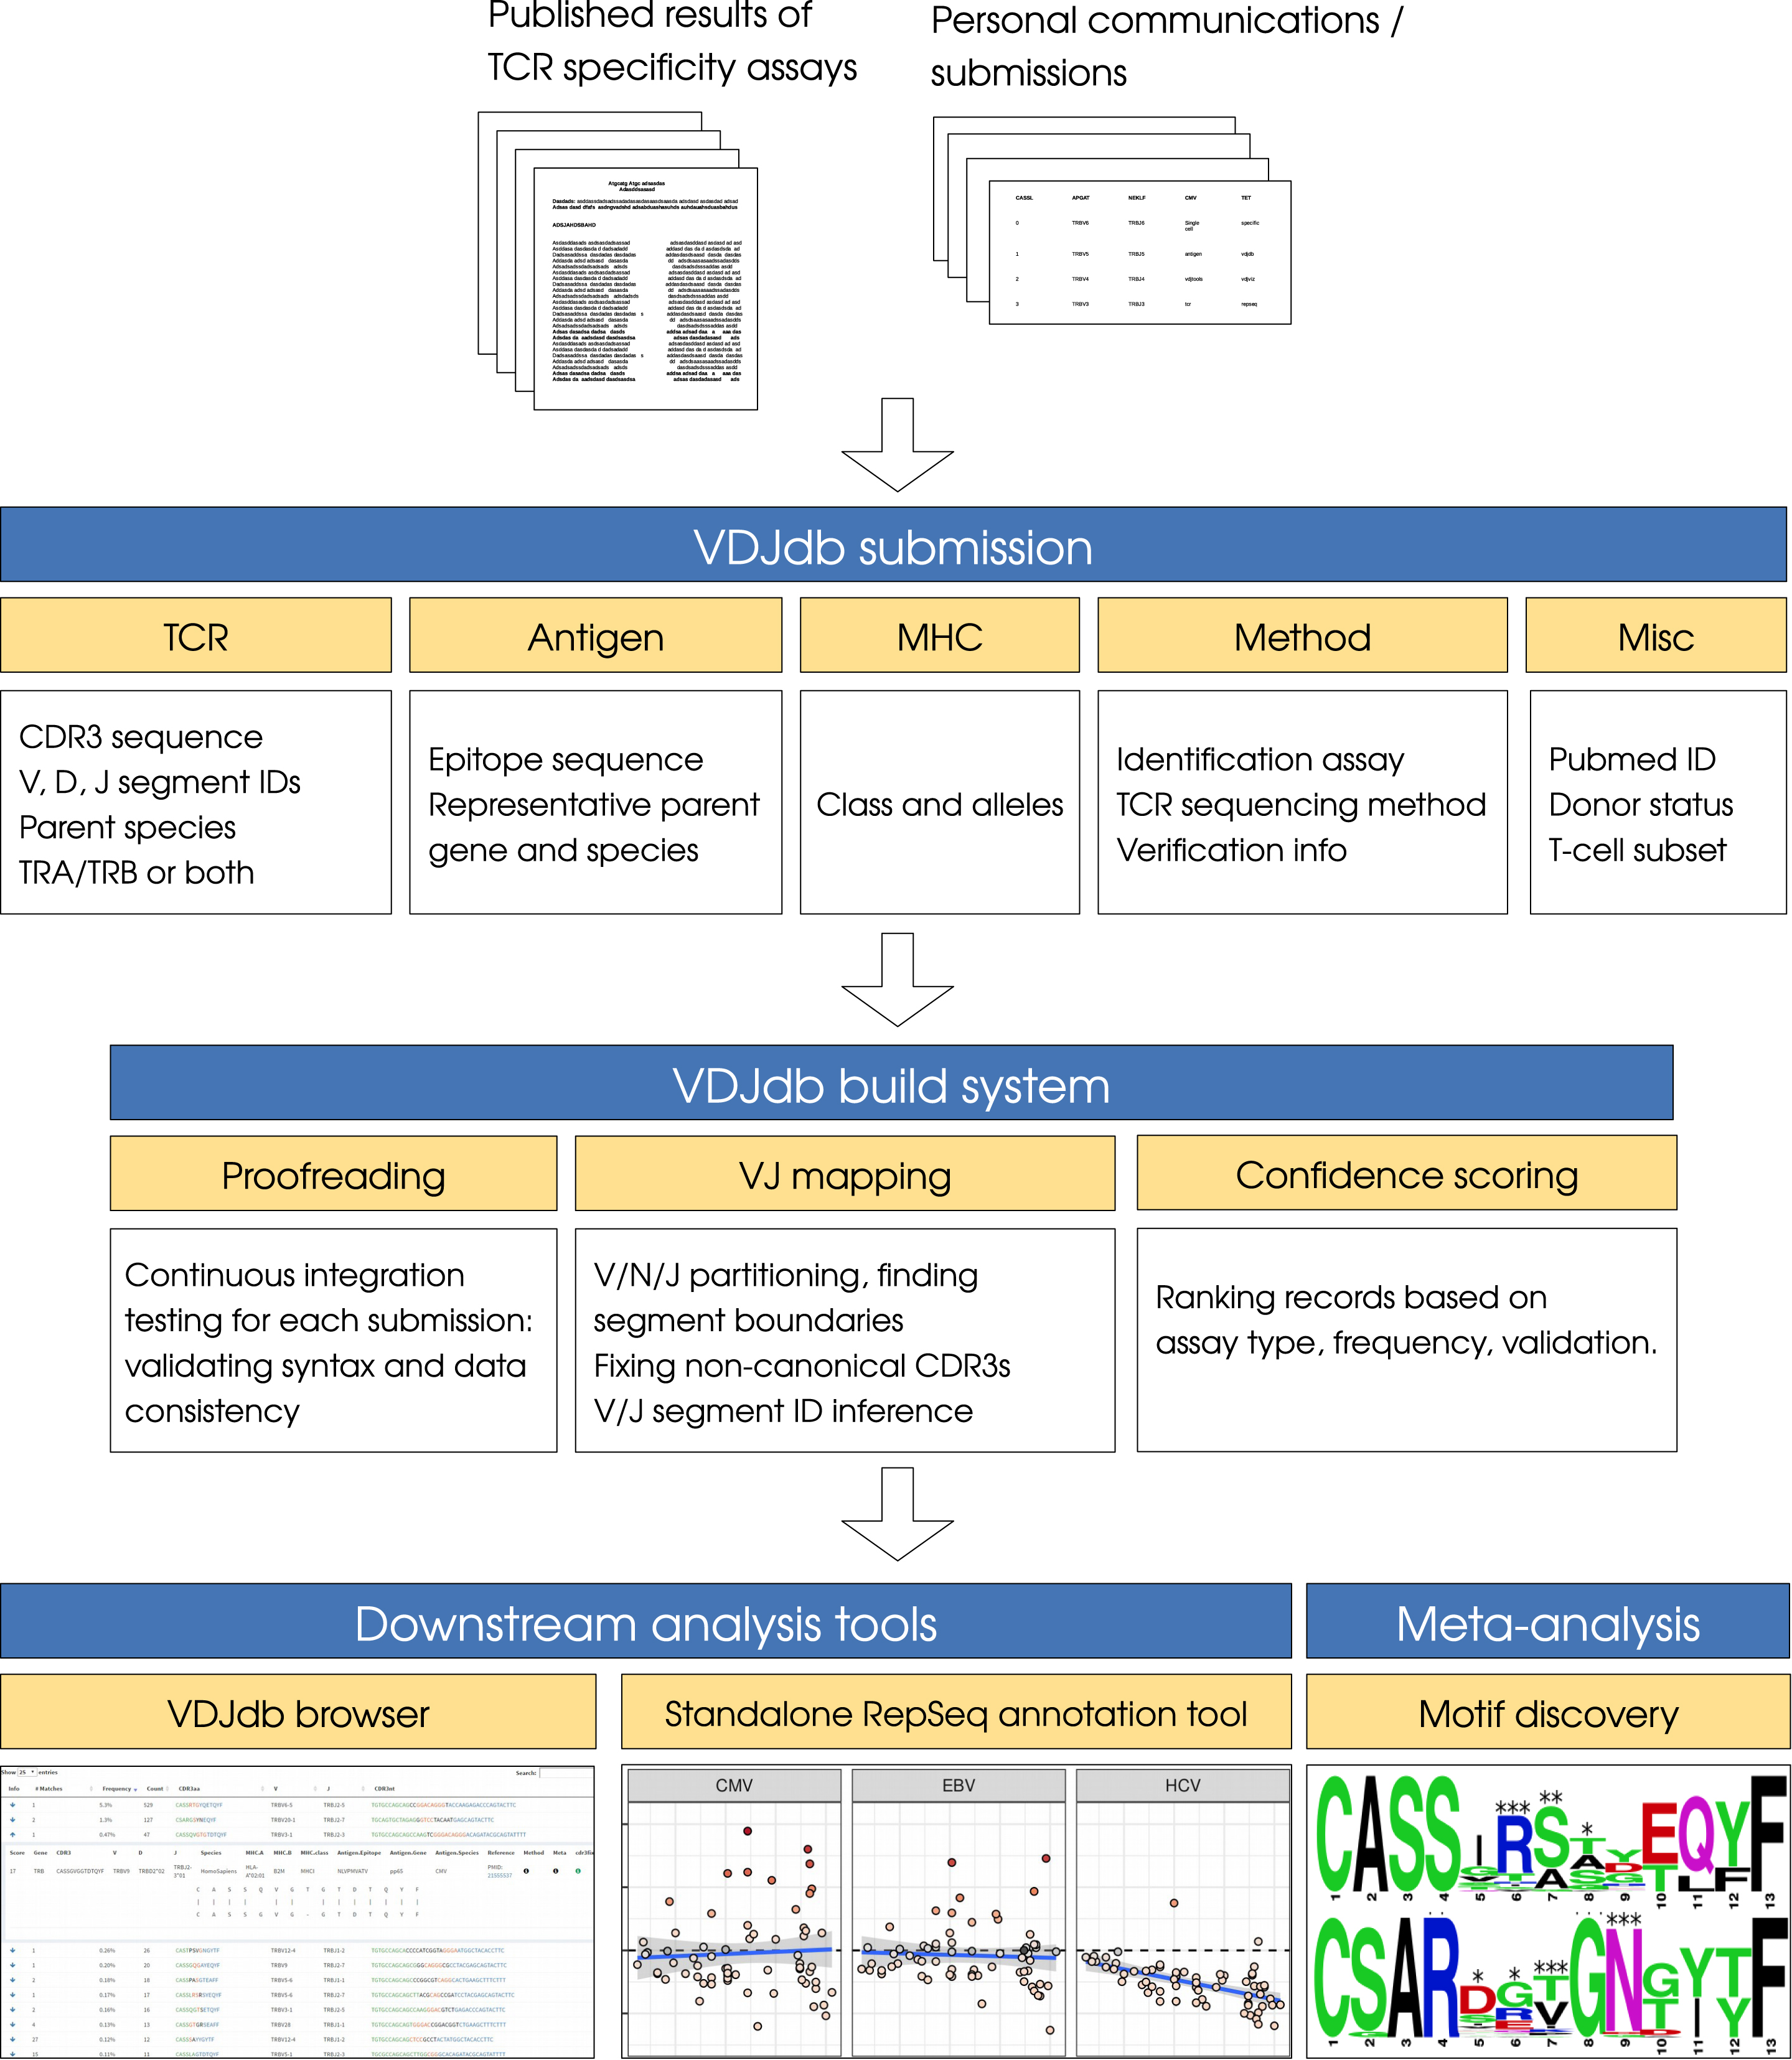
\includegraphics[width=\textwidth]{vdjdb_splash}
\end{columns}
\end{frame}

\begin{frame}{Clonotype tables}
We define a clonotype as a unique combination of Variable (V) and Joining (J) segment and CDR3nt sequence observed in our sequencing data.\\~\

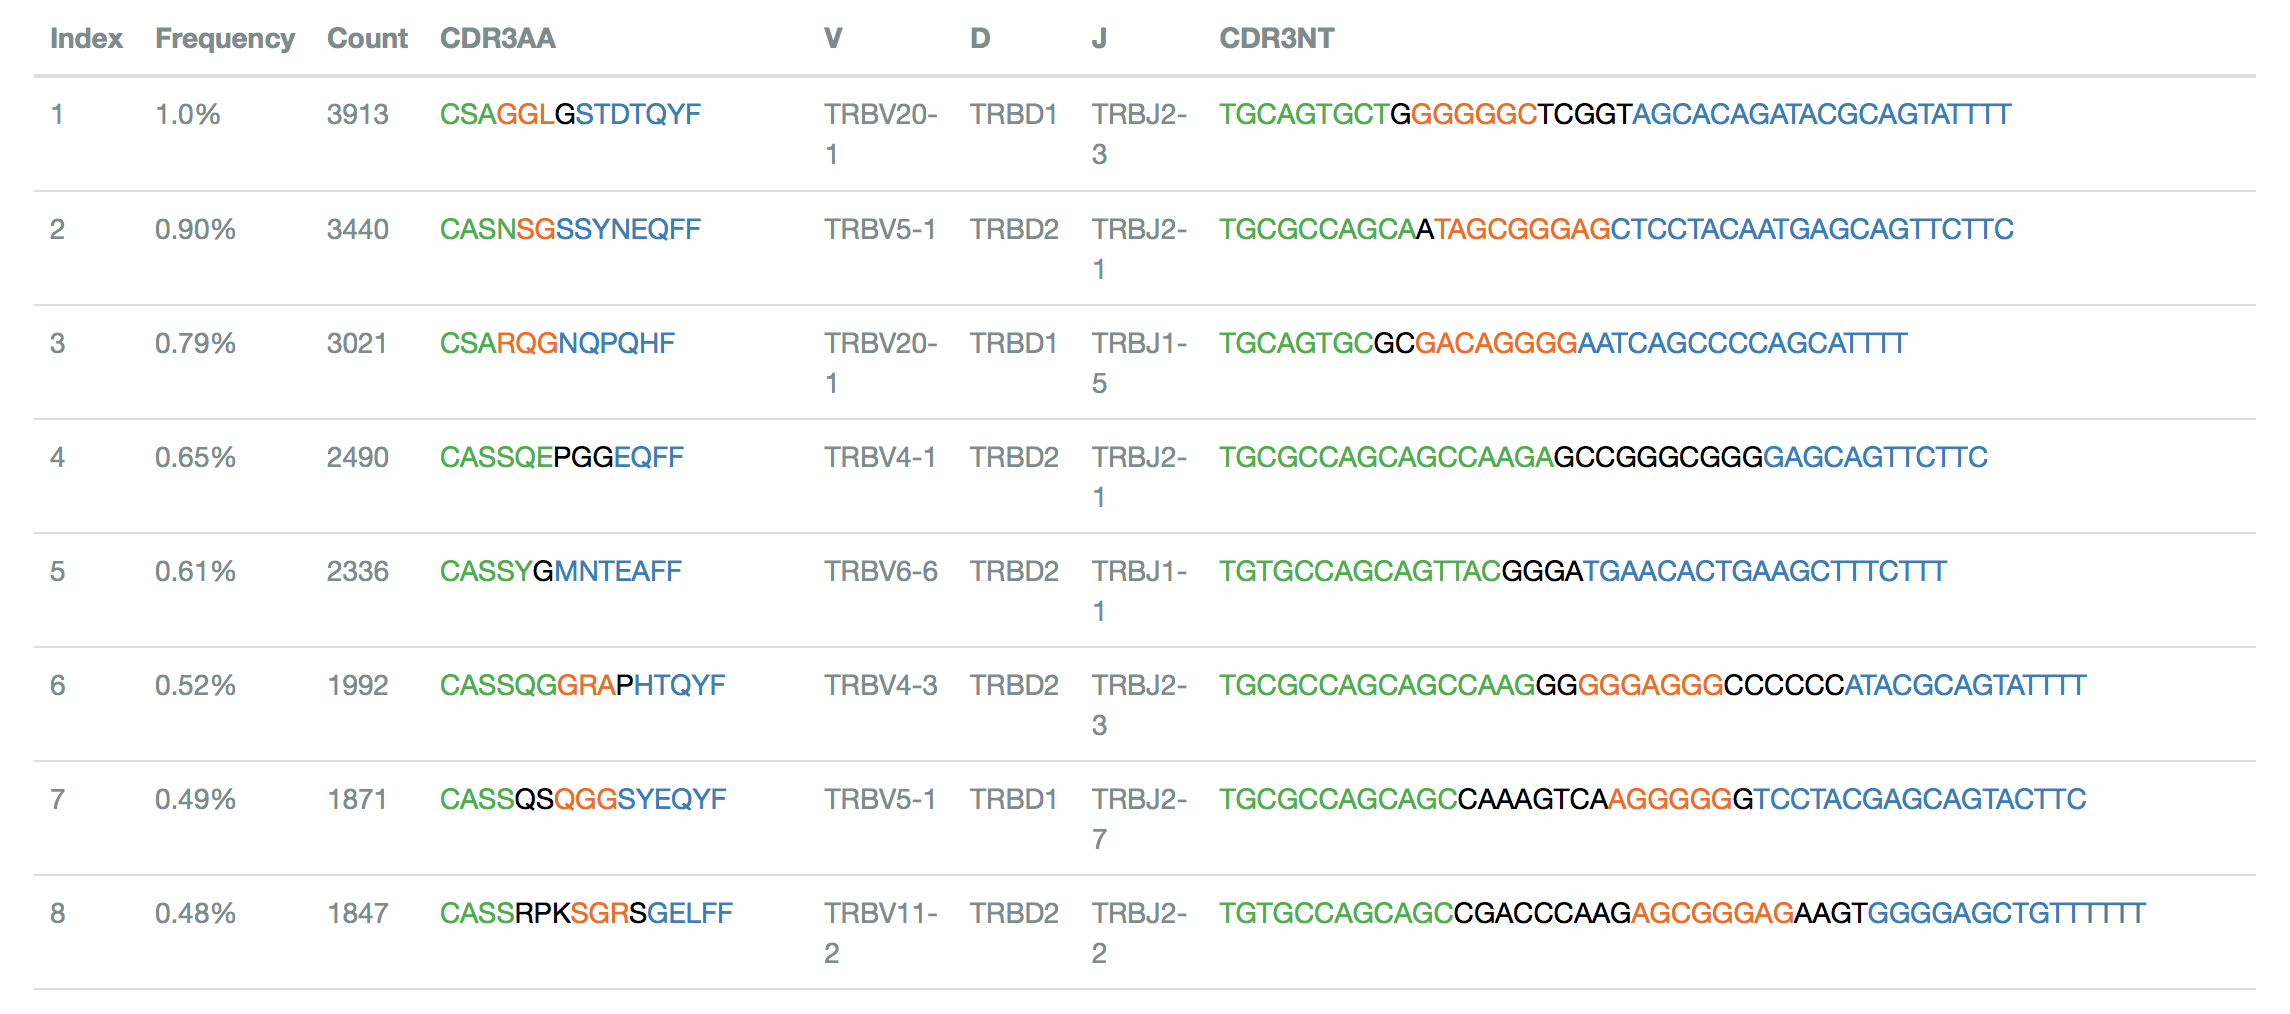
\includegraphics[width=\textwidth]{clonotype_table}
\end{frame}

\begin{frame}{TCR motif inference}
Motif inference in present tutorial is based on the TCR neighbor enrichment test (\texttt{TCRNET}) implemented in \texttt{VDJtools}.\\~\

\texttt{TCRNET} scans TCR sequence graph from a sample of interest and detects nodes having a degree higher than would be expected from placing a given node in the control sample.
\end{frame}

\begin{frame}{Test for TCR neighbor enrichment}
Let $n_i^s$ be the number of clonotypes in sample $s$ that differ from $i$\textsuperscript{th} clonotype by no more than $d=1$ substitutions in the CDR3aa sequence.\footnote{They don't have to have the same V/J segments}\\~\

Let $N_i^s$ be the total number of clonotypes having the same V/J segments as $i$\textsuperscript{th} clonotype in sample $s$.\\~\

Select clonotypes with more neighbors than expected by chance by assuming that

\begin{equation}
n_i^s\stackrel{H_0}{\sim} Poisson\left(N_i^s\frac{n_i^c}{N_i^c}\right)
\end{equation}

where $c$ is the control sample.
\end{frame}

\section{Setting}

\begin{frame}{Dataset}
We'll use RepSeq data from Emerson et al. Nat Genet 2017
\begin{table}[]
\begin{tabular}{lllllll}
\textbf{Sample} & \textbf{ID} & \textbf{a1} & \textbf{a2} & \textbf{b1} & \textbf{b2} & \textbf{status} \\
B35+            & HIP02877    & A*26        & A*33        & B*14        & B*35        & CMV-            \\
CMV+            & HIP13994    & A*02        & A*02        & B*07        & B*44        & CMV+            \\
Control-1       & HIP03484    & A*02        & A*02        & B*07        & B*58        & CMV-            \\
Control-2       & HIP03592    & A*02        & A*32        & B*07        & B*39        & CMV-            \\
Control-3       & HIP04532    & A*02        & A*24        & B*07        & B*51        & CMV-            \\
Control-4       & HIP04576    & A*02        & A*30        & B*07        & B*18        & CMV-           
\end{tabular}
\end{table}
\end{frame}

\begin{frame}{Experiment - 1}
Comparing B35+ sample versus samples without this allele
\begin{table}[]
\begin{tabular}{lllllll}
\textbf{Sample} & \textbf{ID} & \textbf{a1} & \textbf{a2} & \textbf{b1}                  & \textbf{b2}                  & \textbf{status} \\
B35+            & HIP02877    & A*26        & A*33        & B*14                         & \cellcolor[HTML]{FFC702}B*35 & CMV-            \\
CMV+            & HIP13994    & A*02        & A*02        & B*07                         & B*44                         & CMV+            \\
Control-1       & HIP03484    & A*02        & A*02        & \cellcolor[HTML]{9698ED}B*07 & \cellcolor[HTML]{9698ED}B*58 & CMV-            \\
Control-2       & HIP03592    & A*02        & A*32        & \cellcolor[HTML]{9698ED}B*07 & \cellcolor[HTML]{9698ED}B*39 & CMV-            \\
Control-3       & HIP04532    & A*02        & A*24        & \cellcolor[HTML]{9698ED}B*07 & \cellcolor[HTML]{9698ED}B*51 & CMV-            \\
Control-4       & HIP04576    & A*02        & A*30        & \cellcolor[HTML]{9698ED}B*07 & \cellcolor[HTML]{9698ED}B*18 & CMV-           
\end{tabular}
\end{table}
\end{frame}

\begin{frame}{Experiment - 2}
Comparing CMV+ and CMV- samples for A*02 and B*07
\begin{table}[]
\begin{tabular}{lllllll}
\textbf{Sample} & \textbf{ID} & \textbf{a1}                  & \textbf{a2} & \textbf{b1}                  & \textbf{b2} & \textbf{status}              \\
B35+            & HIP02877    & A*26                         & A*33        & B*14                         & B*35        & CMV-                         \\
CMV+            & HIP13994    & \cellcolor[HTML]{FFC702}A*02 & A*02        & \cellcolor[HTML]{FFC702}B*07 & B*44        & \cellcolor[HTML]{FFC702}CMV+ \\
Control-1       & HIP03484    & \cellcolor[HTML]{9698ED}A*02 & A*02        & \cellcolor[HTML]{9698ED}B*07 & B*58        & \cellcolor[HTML]{9698ED}CMV- \\
Control-2       & HIP03592    & \cellcolor[HTML]{9698ED}A*02 & A*32        & \cellcolor[HTML]{9698ED}B*07 & B*39        & \cellcolor[HTML]{9698ED}CMV- \\
Control-3       & HIP04532    & \cellcolor[HTML]{9698ED}A*02 & A*24        & \cellcolor[HTML]{9698ED}B*07 & B*51        & \cellcolor[HTML]{9698ED}CMV- \\
Control-4       & HIP04576    & \cellcolor[HTML]{9698ED}A*02 & A*30        & \cellcolor[HTML]{9698ED}B*07 & B*18        & \cellcolor[HTML]{9698ED}CMV-
\end{tabular}
\end{table}
\end{frame}

\section{Interactive part}

\begin{frame}{Interactive part}
\begin{center}
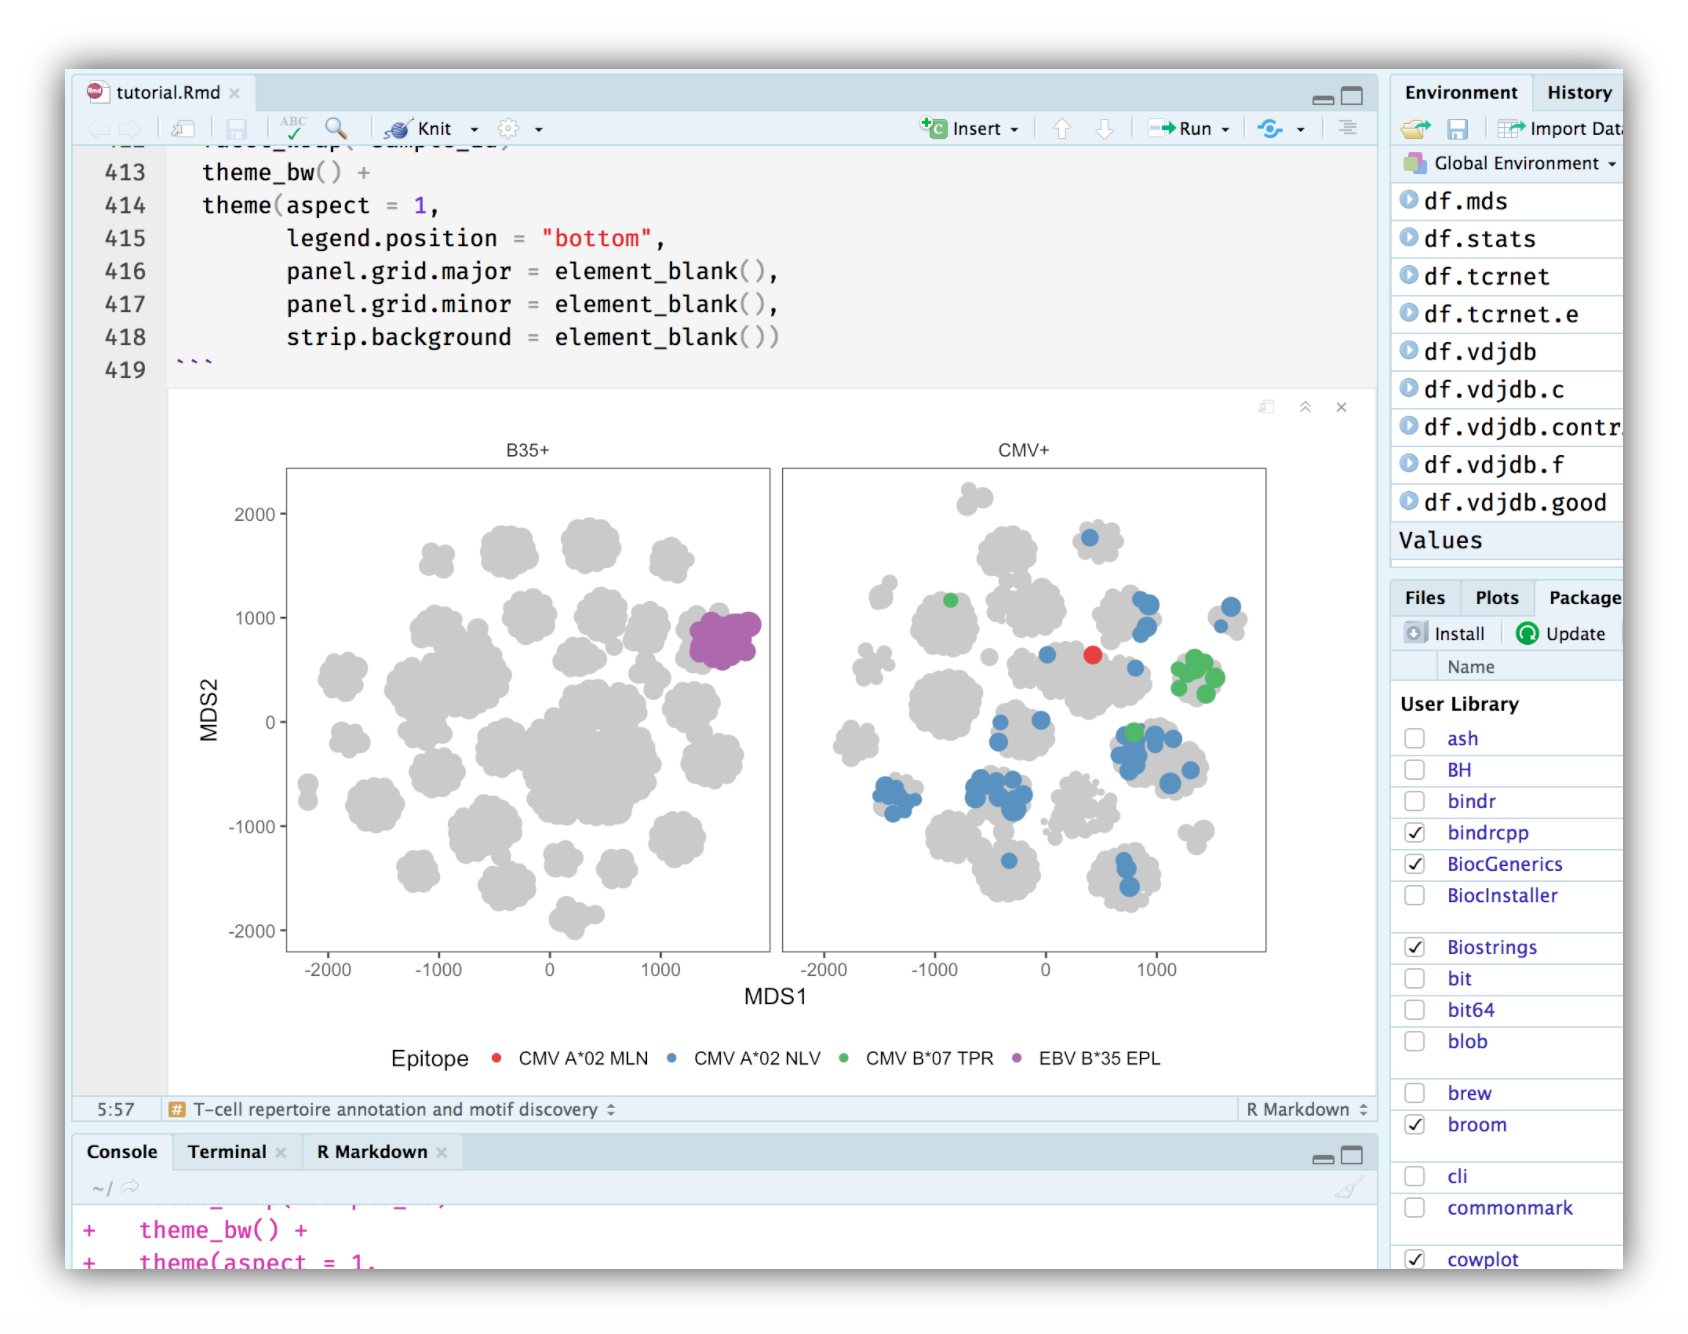
\includegraphics[width=\textwidth]{../splash}
\end{center}
\end{frame}

\section{Concluding remarks}

\begin{frame}{Overview}
\begin{itemize}
\item Annotated our samples with \texttt{VDJdb} and quality-filtered results
\item Filtered annotation results based on our allele of interest (HLA-B35) or donor status (CMV+)
\item Inferred antigen-specific clonotype groups using \texttt{TCRNET} algorithm in \texttt{VDJtools}
\item Overlaped \texttt{VDJdb} annotations and \texttt{TCRNET} results and extract CDR3 sequence motifs
\end{itemize}
\end{frame}

\begin{frame}{Potential pitfalls}
\begin{itemize}
\item Repertoires are extremely diverse making TCR annotation an imbalanced classification problem. Even when matching against \texttt{VDJdb} with high specificity\footnote{According to VDJdb benchmark odds of matching the same epitope given $1$ substitution in CDR3$\beta$ are around $200+$ to $1$} one will observe many false-positives.
\colorbox{yellow!50!white}{Use proper controls, e.g. naive T-cells}
\item \texttt{TCRNET} will fail in some cases simply because the repertoire of T-cells specific to a given antigen is dominated by a single hyperexpanded clonotype.
\colorbox{yellow!50!white}{Always annotate and check large clonotypes}
\end{itemize}
\end{frame}

\begin{frame}{Note on CMV-specific clonotypes}
Diverse repertoire of dissimilar TCRs, individuals are likely to carry a single hyperexpanded clonotype with no subvariants
\begin{center}
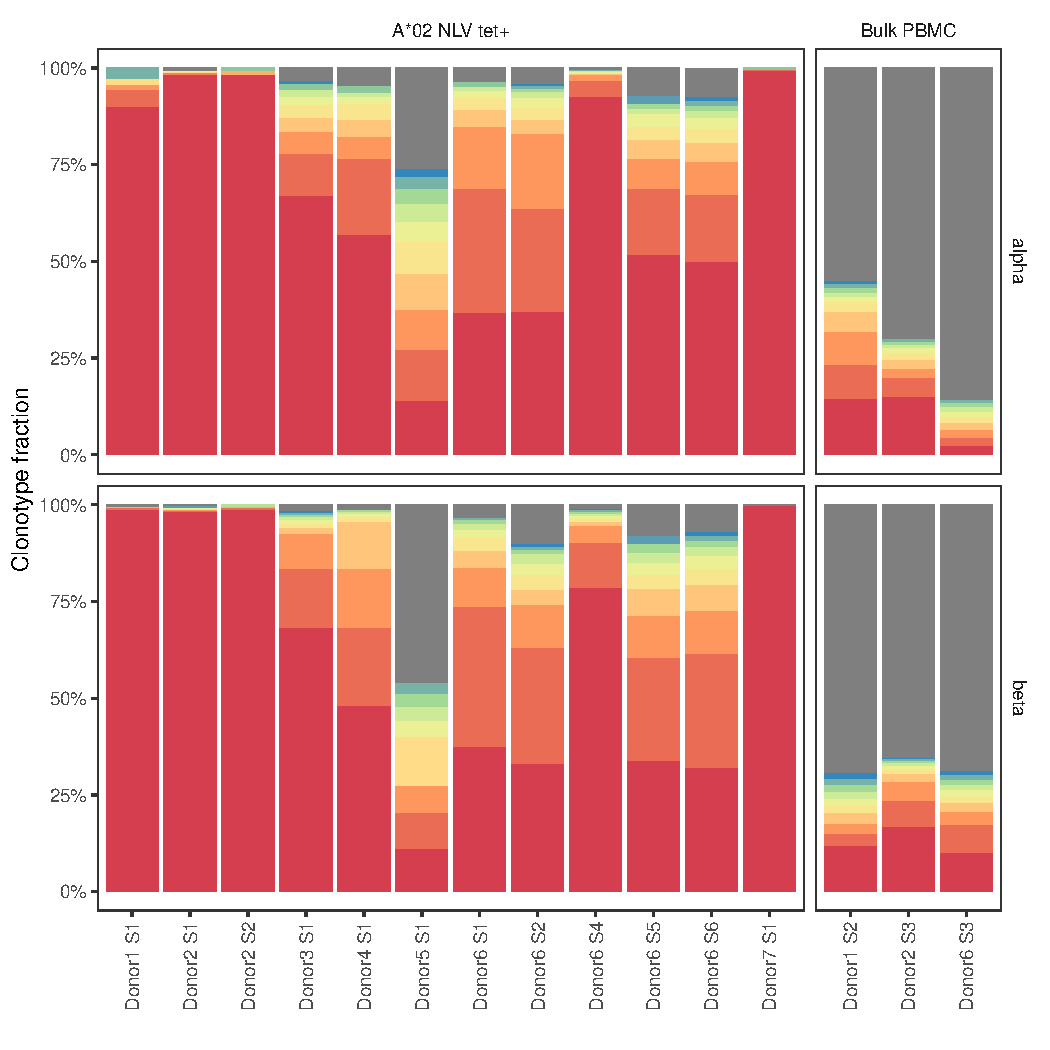
\includegraphics[scale=0.4]{efig0}
\end{center}
\end{frame}

\begin{frame}{}
\centering\Huge\emph{Thank you for listening!}
\end{frame}

\begin{frame}{Contacts}
\begin{itemize}
\Huge\item[\faTwitter]\quad\href{http://twitter.com/antigenomics}{antigenomics}
\Huge\item[\faGithub]\quad\href{https://github.com/mikessh}{mikessh}, \href{https://github.com/antigenomics}{antigenomics}
\Huge\item[\faEnvelope]\quad\href{mailto: mikhail.shugay@gmail.com}{mikhail.shugay@gmail.com}  \\~\
\end{itemize}
\end{frame}

\end{document}